\documentclass[12pt, twocolumn]{article}
\usepackage[utf8]{inputenc}
\usepackage{latexsym}
\usepackage{graphicx}
\usepackage{multicol,multirow}
\usepackage{amsmath,amssymb,amsfonts}
\usepackage{mathrsfs}
\usepackage{amsthm}
\usepackage{rotating}
\usepackage{appendix}
\usepackage[authoryear]{natbib}
\usepackage{ifpdf}
\usepackage[T1]{fontenc}
\usepackage[type1,lining]{ebgaramond}
\usepackage[type1,lining]{sourcesanspro}
\usepackage{newtxmath}
\usepackage{textcomp}%
\usepackage{xcolor}%
\usepackage{hyperref}
\usepackage{lipsum}
\usepackage{polski}
\usepackage{type1cm}
\usepackage{lettrine}

\title{Wielki Trek}
\author{Kamila Kobylańska, Piotr Dyrda, Mikołaj Mężyk}
\date{25 października 2021}

\begin{document}
\maketitle
%\twocolumn
\begin{quote}
  \textit{To właśnie jest nieszczęściem Afrykanerów, jeśli kiedykolwiek coś przedsięwezmą, każdy chce być sam sobie panem i w ten oto sposób wszystko idzie źle.}
  \begin{flushright}
    \tiny{---Carolus Trichardt}
  \end{flushright}
\end{quote}

\section{Wprowadzenie}

\lettrine{W}{ }  połowie XVII wieku, na Przylądku Dobrej Nadziei, Holenderska Kompania Wschodnioindyjska założyła stację zaopatrzeniową. Napływ osadnictwa był powolny, jednakże, pod koniec XVIII wieku, liczba ludności wynosiła kilkanaście tysięcy, a zasięg terytorialny kolonii był bardzo duży, ze względu na niewielki opór lokalnych plemion. \\
W erze napoleońskiej, ze względu na strategiczne położenie, kolonię kilkakrotnie zajmowały siły brytyjskie. Ostatecznie, w 1814 roku, Republika Batawska zrzekła się terytorium na rzecz Wielkiej Brytanii. W 1820 roku rozpoczęto planową akcję brytyjskiej kolonizacji, jednakże pierwsze reformy mające na celu anglicyzację Kolonii Przylądkowej miały miejsce w 1806 roku. Zmiany prawa i napływ Brytyjczyków wywołały niezadowolenie holenderskich osadników. Bardzo dotkliwe dla nich były zmiany w zasadach obrotu ziemią, ponieważ większość osadników nie posiadała formalnych praw własności, oraz zlikwidowanie niewolnictwa. Pomimo, iż mieszkańcy kolonii spodziewali się drugiej zmiany, oburzenie wywołały odszkodowania w~wysokości 50\% planowanej wielkości oraz konieczność odebrania ich w Londynie. Zmiany te sprawiły, że już do 1835 roku około 1500 osadników wyjechało i osiedliło się w okolicach przyszłej Oranii(trasę wszystkich wędrówek przedstawia rysunek \ref{fig1}).

\section{Początek Treku}

\lettrine{G}{} łód ziemi i problemy z brytyjską administracją doprowadziły do exodusu żyjących pół-nomadycznie osadników (fotografia \ref{fig2}). Nieformalne i niezorganizowane grupy pod przywództwem min. Louisa Tregardta czy Andresa Henrika Podgietera wyruszyły na teren pomiędzy rzeką Oranje i~Vaal . Pomimo ustabilizowania się sytuacji w~tym regionie, po fali niepokojów z~czasów imperium Zulusów wodza Czaki, była to tylko stacja pośrednia ich wędrówki do Natalu na wybrzeżu i~Transwalu w interiorze. Doszło jednak do konfliktu z~ndbelskim wodzem Mzilikazim. Wojna została wygrana dzięki rozgromieniu tubylców w bitwie na wzgórzu Vegkop i miażdżącej wygranej komanda Potgietera i Uysa w bitwie w dolinie rzeki Marico, która zmusiła Nbele do odejścia na tereny dzisiejszego Zimbabwe. 

\section{Natal, Transwal i Orania}
\lettrine{P}{} o wygranej w Oranii pionierzy, zwani Voortrekkerami lub Burami, podzielili się na dwie grupy. Jedna poszła do Transwalu, a druga do Natalu. Druga grupa natknęła się na wrogo nastawionych Zulusów, którzy 17 lutego 1838 wymordowali kilkuset osadników zaczynając wojnę bursko-zuluską. Odważne posunięcia taktyczne oraz wykorzystanie taktyki obrony w taborach i konnych oddziałów zwanych komando doprowadziło do wielkiej wygranej nad Blood River (rysunek \ref{fig3}). 600 osadników pod wodzą Andriesa Pretoriusa odparło armię liczącą do 20 000 wojowników nie tracąc ani jednego człowieka, przy stratach Zuluskich wynoszących około 3 000. Bunt M’Pandy przeciw wodzowi Dinganowi i zajęcie stolicy Zulusów zakończyło wojnę i doprowadziło do powstania Republiki Natalii w~1839r. Jednakże, już w 1842r. doszło do brytyjskiej interwencji i włączenia Natalu do Kolonii Przylądkowej trzy lata później. Doprowadziło to do fali wędrówek do Oranii, również niepokojonej przez siły brytyjskie, oraz Transwalu, która istniał na pograniczu terenów brytyjskich i portugalskich (Mozambik). Ostatecznie wędrówki Burów zakończyły się w 1848r.
\newpage

\section{Skutki}
\lettrine{W}{} ędrówki Voortrekkerów doprowadziły do powstania dwóch państw burskich – Wolnego Państwa Orania i Republiki Natalu. Ugruntowało to tożsamość narodową Burów, doprowadziło do skonsolidowania sił w interiorze i powstania nielicznych, silnych państw burskich i afrykańskich. Otworzyło to również drogę w głąb południa Afryki misjonarzom i podróżnikom, jak choćby David Livingstone. Burowie zagospodarowali interior zniszczony wojnami Zulusów Czaki (okres Mfecane), które doprowadziły do śmierci i migracji milionów. Przejęto znaczną część regionu z rąk tubylców.  

\section{Bibliografia}
\begin{enumerate}
    \item Wielki Trek - Wikipedia [online] 
    \tiny{https://pl.wikipedia.org/wiki/Wielki\_Trek}\normalsize{
    \item What was The Great Trek? - History with Hilbert [online - YouTube]} \tiny{https://www.youtube.com/watch?v=028OjMGirj0\&ab\_channel=HistoryWithHilbert}\normalsize{
    \item Great Trek 1835-1846 - South African History Online [online]} \tiny{https://www.sahistory.org.za/article/great-trek-1835-1846?fbclid=IwAR0sfBT8sM4efLk\_kO-PMo1m0q9vdD64WsCYYF8j2SusPRCiONswqQTCh9k}
\end{enumerate}



\begin{figure}[h]%
\caption{Mapa wędrówek}
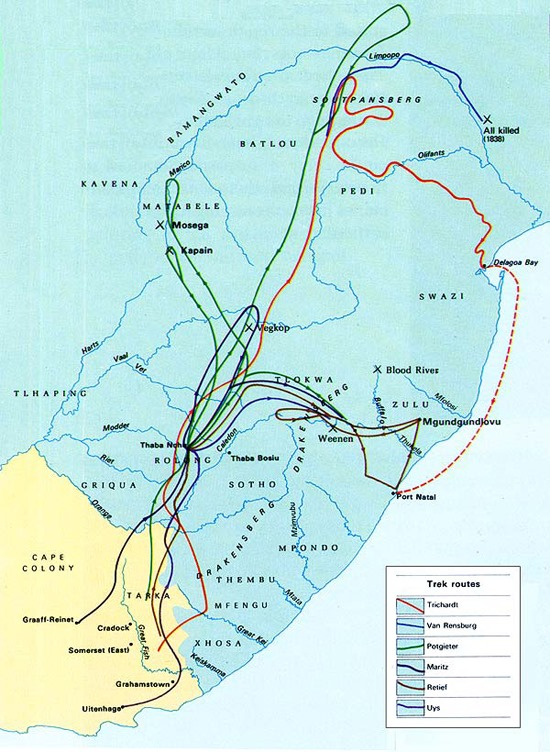
\includegraphics[scale=.8]{mapa.jpg}
\tiny{https://www.tokencoins.com/oompaul.htm}
\label{fig1}
\end{figure}

\onecolumn
\begin{figure}[t]%
\caption{Wygląd przeciętnej rodziny Burów}
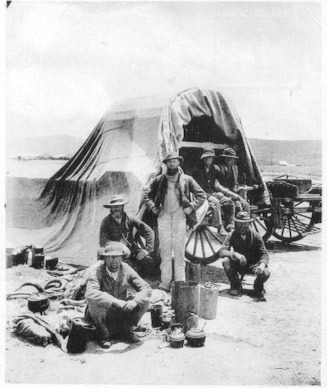
\includegraphics[scale=.6]{Burowie.jpg}
\tiny{https://murderiseverywhere.blogspot.com/2010/10/}
\label{fig2}
\end{figure}

\begin{figure}[p]%
\caption{Bitwa nad Blood River}
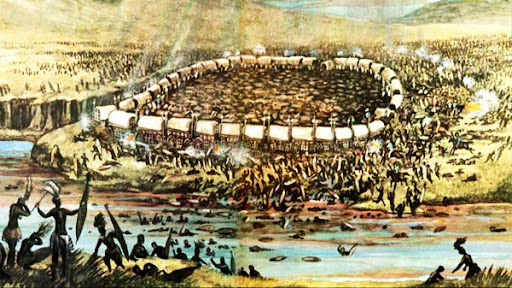
\includegraphics[scale=.8]{blood River.jpg}
\tiny{http://why-we-are-white-refugees.blogspot.com/2009/12/16-december-1838-battle-of-blood-river.html}
\label{fig3}
\end{figure}



\end{document}
